\documentclass[11pt,letterpaper]{article}

% Packages
\usepackage[margin=0.85in]{geometry}
\usepackage{fontspec}
\usepackage{xcolor}
\usepackage{tikz}
\usetikzlibrary{patterns,shapes.geometric,positioning}
\usepackage{tcolorbox}
\usepackage{enumitem}
\usepackage{graphicx}
\usepackage{setspace}
\usepackage{parskip}
\usepackage{multicol}
\usepackage[hidelinks]{hyperref}

% Font setup
\setmainfont{ElMessiri-Regular}[
    Path = ../../assets/fonts/,
    Extension = .ttf,
    BoldFont = ElMessiri-Regular,
    BoldFeatures = {FakeBold=1.5},
    Scale=1.0
]

% Define colors
\definecolor{purple}{RGB}{138,43,226}
\definecolor{blue}{RGB}{30,144,255}
\definecolor{green}{RGB}{34,139,34}
\definecolor{red}{RGB}{220,20,60}
\definecolor{orange}{RGB}{255,140,0}
\definecolor{lightgray}{RGB}{245,245,245}
\definecolor{darkgray}{RGB}{100,100,100}
\definecolor{mediumgray}{RGB}{150,150,150}

% Custom commands for colored text
\newcommand{\purple}[1]{\textcolor{purple}{\textbf{#1}}}
\newcommand{\bluepurple}[1]{\textcolor{blue}{\textbf{#1}}}
\newcommand{\greentext}[1]{\textcolor{green}{\textbf{#1}}}
\newcommand{\redtext}[1]{\textcolor{red}{\textbf{#1}}}
\newcommand{\orangetext}[1]{\textcolor{orange}{\textbf{#1}}}

% Header and footer
\usepackage{fancyhdr}
\pagestyle{fancy}
\fancyhf{}
\renewcommand{\headrulewidth}{0.4pt}
\renewcommand{\footrulewidth}{0.4pt}
\fancyhead[L]{\small\textit{Music Theory \& Terminology Handbook}}
\fancyhead[R]{\small\textit{Beatmaking: Learn By Doing}}
\fancyfoot[C]{\small\thepage}

% Title formatting
\usepackage{titlesec}
\titleformat{\section}
  {\LARGE\bfseries\sffamily\color{purple}}
  {}
  {0em}
  {}
  [\vspace{-0.5em}\rule{\textwidth}{0.5pt}]
\titleformat{\subsection}
  {\Large\bfseries\sffamily\color{blue}}
  {}
  {0em}
  {}
\titleformat{\subsubsection}
  {\large\bfseries\sffamily\color{darkgray}}
  {}
  {0em}
  {}

% Better spacing
\setlength{\parskip}{0.6em}
\setstretch{1.15}

% Table of contents formatting
\usepackage{tocloft}
\renewcommand{\cftsecfont}{\bfseries\sffamily}
\renewcommand{\cftsubsecfont}{\sffamily}

\begin{document}

% ============================================================================
% TITLE PAGE
% ============================================================================

\thispagestyle{empty}

\vspace*{\fill}

\begin{center}
{\Huge\bfseries\sffamily Music Theory \& Terminology}

\vspace{0.3cm}

{\LARGE\bfseries\sffamily Handbook for Beginners}

\vspace{0.5cm}


\begin{tikzpicture}
    % Decorative music notes
    \fill[purple] (0,0) circle (0.25cm);
    \draw[purple, line width=2pt] (0.25,0) -- (0.25,1.2);
    \fill[blue] (1.2,0.2) circle (0.25cm);
    \draw[blue, line width=2pt] (1.45,0.2) -- (1.45,1.4);
    \fill[green] (2.4,0) circle (0.25cm);
    \draw[green, line width=2pt] (2.65,0) -- (2.65,1.2);
    \fill[orange] (3.6,0.2) circle (0.25cm);
    \draw[orange, line width=2pt] (3.85,0.2) -- (3.85,1.4);
\end{tikzpicture}

\vspace{0.8cm}

{\Large\textit{A Simple, Modern Guide for Beatmakers \& Producers}}

\vspace{1cm}

\begin{tcolorbox}[colback=lightgray,colframe=purple,width=0.8\textwidth,arc=3mm,boxrule=1.5pt]
\begin{center}
\textbf{From absolute beginner to confident creator}

\vspace{0.3cm}

Learn the language of music through a \\
\purple{beatmaker's perspective}
\end{center}
\end{tcolorbox}

\end{center}

\vspace*{\fill}

\begin{center}
\rule{0.8\textwidth}{0.5pt}

\vspace{0.3cm}

\textbf{Beatmaking: Learn By Doing}

\textit{Learn music through \purple{beats} — A fun, \bluepurple{human} path to modern music making}

\vspace{0.3cm}

\small www.makebeatsanywhere.com | @the\_beat\_machine\_

\vspace{0.3cm}

\rule{0.8\textwidth}{0.5pt}
\end{center}

\newpage

% ============================================================================
% TABLE OF CONTENTS
% ============================================================================

\tableofcontents

\newpage

% ============================================================================
% INTRODUCTION
% ============================================================================

\section*{How to Use This Handbook}
\addcontentsline{toc}{section}{How to Use This Handbook}

Welcome to your music theory handbook! This isn't your typical theory textbook. We're skipping the boring stuff and focusing on what you actually need to know to start making beats.

\subsection*{Who Is This For?}

This handbook is for \textbf{complete beginners}—people who want to make music but don't know where to start. Maybe you've never touched an instrument. Maybe you don't know what a "chord" is. That's perfect. We're starting from zero.

\subsection*{The Beatmaker's Perspective}

Traditional music theory books teach you like you're going to become a classical composer. That's not us. We're teaching you theory the way modern producers and beatmakers need it:

\begin{itemize}[leftmargin=*]
\item \textbf{Simple} - no unnecessary jargon
\item \textbf{Practical} - focused on what you'll actually use
\item \textbf{Modern} - written for DAWs, MIDI, and digital production
\item \textbf{Action-oriented} - every concept includes how to apply it
\end{itemize}

\subsection*{How It's Organized}

This handbook is organized from foundation to application:

\begin{enumerate}[leftmargin=*]
\item \textbf{Building Blocks} - Rhythm and time (beats, BPM, drums)
\item \textbf{Pitch} - High and low (notes, scales, keys)
\item \textbf{Harmony} - Notes together (intervals, chords, progressions)
\item \textbf{Beatmaker's Toolkit} - Your instruments (drums, bass, keys)
\item \textbf{Song Structure} - Arranging your ideas
\item \textbf{Production Basics} - Essential DAW and mixing terms
\item \textbf{Techniques} - Compositional and groove concepts
\item \textbf{Appendices} - Quick reference charts and glossary
\end{enumerate}

\subsection*{Reading Tips}

\begin{tcolorbox}[colback=blue!5,colframe=blue,width=\textwidth,arc=3mm,boxrule=1pt]
Throughout this handbook, you'll see sections organized like this:

\textbf{\purple{What It Is:}} A simple, clear definition

\textbf{\bluepurple{Why It Matters:}} How this helps you make better beats

\textbf{\greentext{In Real Songs:}} Examples from actual music

\textbf{\orangetext{Try It Yourself:}} Something you can do right now
\end{tcolorbox}

You don't have to read this cover-to-cover. Use it as a reference. Look up terms when you encounter them. Skim the parts that interest you most.

\subsection*{The Goal}

By the end of this handbook, you'll understand the fundamental language of music. You'll be able to talk about beats, notes, chords, and arrangements with confidence. More importantly, you'll be able to \textbf{apply} these concepts to create your own music.

Let's get started.

\newpage

% ============================================================================
% PART 1: THE BUILDING BLOCKS OF SOUND
% ============================================================================

\section{Part 1: The Building Blocks of Sound}

Music has two fundamental elements: \purple{rhythm} (time) and \bluepurple{pitch} (highness/lowness). Before we dive into complicated theory, let's understand what music actually is and start with rhythm—the heartbeat of every beat.

% ----------------------------------------------------------------------------
% CHAPTER 1: WHAT IS MUSIC?
% ----------------------------------------------------------------------------

\subsection{Chapter 1: What Is Music?}

\subsubsection{Sound}

Everything starts with \textbf{sound}—vibrations traveling through the air that your ear picks up. When something vibrates (a drum head, a guitar string, your vocal cords), it creates waves in the air. Those waves hit your eardrum, and your brain interprets them as sound.

\textbf{\purple{What It Is:}} Sound is physical vibrations traveling through air (or water, or solid objects).

\textbf{\bluepurple{Why It Matters:}} Understanding that sound is vibration helps you understand why bass "hits" harder (bigger, slower vibrations) and why high notes feel sharper (faster vibrations).

\subsubsection{Music vs. Noise}

So what's the difference between music and noise?

\textbf{Music} is organized sound with intention. It has patterns, rhythm, structure. When you tap your fingers on a table randomly, that's just noise. When you tap them in a steady pattern—boom, tap, boom, tap—that's the beginning of music.

\textbf{Noise} is random, chaotic sound without pattern or organization.

The cool thing? The line between music and noise is flexible. What sounds like noise to one person might be music to another. Some of the most innovative music uses sounds that were traditionally considered "noise."

\subsubsection{The Two Big Elements}

All music—from classical symphonies to trap beats—is built on two fundamental elements:

\begin{enumerate}[leftmargin=*]
\item \textbf{\redtext{Rhythm} (Time)} - When sounds happen
\begin{itemize}
\item The beat, the groove, the timing
\item How fast or slow
\item The pattern of hits and spaces
\end{itemize}

\item \textbf{\bluepurple{Pitch} (Highness/Lowness)} - How high or low sounds are
\begin{itemize}
\item Notes, melodies, chords
\item Bass (low) vs. lead (high)
\item Harmony and melody
\end{itemize}
\end{enumerate}

\begin{tcolorbox}[colback=orange!10,colframe=orange,width=\textwidth,arc=3mm,boxrule=1pt]
\textbf{\orangetext{Try It Yourself:}}

Close your eyes and listen to a song—any song. First, focus only on the rhythm. Tap along with the beat. Ignore the melody and chords. Just feel the pulse and pattern.

Now listen again, but this time focus only on the pitch. Ignore the rhythm. Listen to how notes move up and down, how high or low things are.

Notice how both elements work together to create the complete musical experience.
\end{tcolorbox}

\newpage

% ----------------------------------------------------------------------------
% CHAPTER 2: RHYTHM - THE HEARTBEAT
% ----------------------------------------------------------------------------

\subsection{Chapter 2: Rhythm — The Heartbeat}

Rhythm is the foundation of beatmaking. Before you worry about chords or melodies, you need to understand time and rhythm. This is where it all begins.

\subsubsection{The Beat}

The \textbf{beat} is the steady pulse of music—the thing you nod your head to, the thing that makes you want to move.

\textbf{\purple{What It Is:}} A steady, repeating pulse. Think of it like a heartbeat or a ticking clock. Boom. Boom. Boom. Boom.

\textbf{\bluepurple{Why It Matters:}} The beat is the foundation of your entire track. Everything else—drums, bass, melody—locks into this steady pulse.

\textbf{\greentext{In Real Songs:}} 
\begin{itemize}[leftmargin=*]
\item In "Still D.R.E.," the beat is that steady, head-nodding pulse at 93 BPM
\item In "Levels," the beat is faster and more energetic at 126 BPM
\item In "Come Together," the beat is slow and swampy at 82 BPM
\end{itemize}

\textbf{\orangetext{Try It Yourself:}} Put on any song and tap your foot to the steady pulse. Don't overthink it—just find the pulse that makes you want to move. That's the beat.

\subsubsection{BPM (Beats Per Minute)}

\textbf{BPM} tells you how fast or slow the beat is. It literally means "beats per minute"—how many pulses happen in 60 seconds.

\textbf{\purple{What It Is:}} The speed of the beat, measured in pulses per minute.

\begin{itemize}[leftmargin=*]
\item \textbf{Slow (60-90 BPM)} - Chill, laid-back, emotional
  \begin{itemize}
  \item Hip-hop often sits here (70-95 BPM)
  \item "Come Together" by The Beatles: 82 BPM
  \item Feels relaxed, room to breathe
  \end{itemize}

\item \textbf{Medium (90-120 BPM)} - Walking pace, groove-oriented
  \begin{itemize}
  \item Funk, soul, mid-tempo pop
  \item "Still D.R.E." by Dr. Dre: 93 BPM
  \item The sweet spot for head-nodding grooves
  \end{itemize}

\item \textbf{Fast (120-140 BPM)} - Energetic, dance-oriented
  \begin{itemize}
  \item House, techno, pop, EDM
  \item "Levels" by Avicii: 126 BPM
  \item Makes you want to dance
  \end{itemize}

\item \textbf{Very Fast (140-180+ BPM)} - Intense, high-energy
  \begin{itemize}
  \item Drum \& bass (160-180 BPM)
  \item Trap (often 140-150 BPM but feels half as fast)
  \item Aggressive, intense energy
  \end{itemize}
\end{itemize}

\textbf{\bluepurple{Why It Matters:}} BPM sets the vibe of your entire track. Slow BPM = chill and emotional. Fast BPM = energetic and dance-y. Choose your BPM based on the feeling you want.

\textbf{\orangetext{Try It Yourself:}} Open your DAW and set it to 80 BPM. Create a simple kick drum pattern. Now change it to 120 BPM. Same pattern, totally different energy. Feel the difference.

\subsubsection{Bar / Measure}

Beats are organized into groups called \textbf{bars} (also called \textbf{measures}).

\textbf{\purple{What It Is:}} A bar is a group of beats—almost always 4 beats. 

Count along with a song: "1, 2, 3, 4 | 1, 2, 3, 4 | 1, 2, 3, 4..." Each time you count to 4, that's one bar.

\textbf{\bluepurple{Why It Matters:}} Bars are the building blocks of your song structure. You'll think in terms of bars:
\begin{itemize}[leftmargin=*]
\item "Let's add 8 bars of just drums"
\item "The verse is 16 bars long"
\item "Switch the pattern every 4 bars"
\end{itemize}

Most music is organized in groups of 4 bars (16 beats), 8 bars (32 beats), or 16 bars (64 beats).

\begin{tcolorbox}[colback=lightgray,colframe=purple,width=\textwidth,arc=3mm,boxrule=1pt]
\textbf{Pro Tip:} In your DAW, the timeline is divided into bars. When you see "Bar 1," "Bar 2," "Bar 3"—those are your measures. Most DAWs also show the beat within each bar: "1.1" means Bar 1, Beat 1. "2.3" means Bar 2, Beat 3.
\end{tcolorbox}

\subsubsection{The Drum Kit: Kick, Snare, Hi-Hat}

Now let's talk about the three core drums that create the basic beat pattern:

\textbf{1. Kick (Bass Drum)}

\textbf{\purple{What It Is:}} The kick is the lowest drum—the big "boom" you feel in your chest. It's usually the deepest, most powerful sound in your beat.

\textbf{\bluepurple{Why It Matters:}} The kick is the foundation. It usually hits on beats 1 and 3 (or on all four beats). It works with the bass to create the low-end power.

\textbf{\greentext{In Real Songs:}}
\begin{itemize}[leftmargin=*]
\item "Come Together" - Sparse kick on beats 1 and 3
\item "Still D.R.E." - Steady four-on-the-floor (kick on every beat: 1, 2, 3, 4)
\item "Levels" - Four-on-the-floor with that signature EDM pump
\end{itemize}

\vspace{0.3cm}

\textbf{2. Snare}

\textbf{\purple{What It Is:}} The snare is the sharp, cracking sound—like a whip. It's higher-pitched than the kick and cuts through the mix.

\textbf{\bluepurple{Why It Matters:}} The snare creates the "backbeat"—it usually hits on beats 2 and 4. This is what makes you want to clap along to music.

When you clap along to a song, you're almost always clapping on the snare hits (beats 2 and 4).

\textbf{\greentext{In Real Songs:}} In almost every song, the snare (or clap) hits on 2 and 4. That's the universal pattern that drives rhythm across nearly all genres.

\vspace{0.3cm}

\textbf{3. Hi-Hat}

\textbf{\purple{What It Is:}} The hi-hat is the metallic, ticking sound—like "tss-tss-tss." It's the highest-pitched element of the drum kit.

\textbf{\bluepurple{Why It Matters:}} The hi-hat subdivides the beat, adding energy and movement. It can play on every beat, every half-beat (8th notes), or even faster (16th notes).

\textbf{Closed Hi-Hat:} Tight, short sound (tss)
\textbf{Open Hi-Hat:} Longer, ringing sound (tsssss)

The hi-hat creates the groove and texture. Slow, steady hi-hats feel relaxed. Fast, intricate hi-hat patterns feel energetic.

\subsubsection{The Basic Beat Pattern}

Here's the most fundamental beat pattern in all of music:

\begin{tcolorbox}[colback=red!5,colframe=red,width=\textwidth,arc=3mm,boxrule=1pt]
\textbf{The Universal Beat Pattern:}

\begin{itemize}[leftmargin=*]
\item \textbf{Kick:} Beats 1 and 3 (or all four beats)
\item \textbf{Snare:} Beats 2 and 4
\item \textbf{Hi-Hat:} Every beat (or every half-beat for more energy)
\end{itemize}

\vspace{0.3cm}

Count it out:

\begin{center}
\textbf{1} (Kick + Hi-Hat) \quad \textbf{2} (Snare + Hi-Hat) \quad \textbf{3} (Kick + Hi-Hat) \quad \textbf{4} (Snare + Hi-Hat)
\end{center}

This is the foundation of rock, pop, hip-hop, funk, house—almost every genre.
\end{tcolorbox}

\textbf{\orangetext{Try It Yourself:}} 

Open your DAW and create three tracks: Kick, Snare, Hi-Hat.

\begin{enumerate}[leftmargin=*]
\item Put kick drums on beats 1 and 3
\item Put snares on beats 2 and 4  
\item Put hi-hats on every beat (1, 2, 3, 4)
\end{enumerate}

Loop it. Congratulations—you just made a beat! Now experiment:
\begin{itemize}[leftmargin=*]
\item Try kick on every beat (four-on-the-floor)
\item Try hi-hats on every half-beat (twice as fast)
\item Try removing the kick on beat 3
\end{itemize}

Small changes create completely different grooves.

\newpage

% ----------------------------------------------------------------------------
% CHAPTER 3: TIME AND RHYTHM NOTATION
% ----------------------------------------------------------------------------

\subsection{Chapter 3: Time and Rhythm Notation}

Now that you understand the beat, let's talk about how beats are divided and how to read rhythm in your DAW.

\subsubsection{Time Signature}

The \textbf{time signature} tells you how many beats are in each bar and what type of note gets one beat.

\textbf{\purple{What It Is:}} A fraction-like symbol (like 4/4) that defines the rhythmic structure.

The most common time signature is \textbf{4/4} (pronounced "four-four" or "common time"):
\begin{itemize}[leftmargin=*]
\item Top number (4) = 4 beats per bar
\item Bottom number (4) = A quarter note gets one beat
\end{itemize}

\textbf{\bluepurple{Why It Matters:}} 99\% of modern music uses 4/4 time. This is why we count "1, 2, 3, 4" and why almost everything is organized in groups of 4.

\begin{tcolorbox}[colback=lightgray,colframe=darkgray,width=\textwidth,arc=3mm,boxrule=1pt]
\textbf{Other Time Signatures (You'll Rarely See These):}

\textbf{3/4} - Three beats per bar (waltz feel: "1, 2, 3 | 1, 2, 3")

\textbf{6/8} - Six beats per bar with a triplet feel (think slow ballads)

Don't worry about these yet. Stick with 4/4 for now—that's where 99\% of beats live.
\end{tcolorbox}

\subsubsection{Note Lengths}

Notes can be different lengths. Here's how beats are divided:

\textbf{Whole Note} - 4 beats (the entire bar)
\begin{itemize}[leftmargin=*]
\item Hold for the full bar
\item Rarely used in beatmaking except for long pad sounds
\end{itemize}

\textbf{Half Note} - 2 beats
\begin{itemize}[leftmargin=*]
\item Halfway through a bar
\item Useful for bass notes and chord changes
\end{itemize}

\textbf{Quarter Note} - 1 beat ← \textbf{THIS IS THE MAIN BEAT}
\begin{itemize}[leftmargin=*]
\item When you count "1, 2, 3, 4," each number is a quarter note
\item Most kick and snare patterns use quarter notes
\item This is your primary reference point
\end{itemize}

\textbf{8th Note} - Half a beat (0.5 beats)
\begin{itemize}[leftmargin=*]
\item The "and" between beats: "1-and-2-and-3-and-4-and"
\item Common for hi-hats and rhythmic patterns
\item Twice as fast as quarter notes
\end{itemize}

\textbf{16th Note} - Quarter of a beat (0.25 beats)
\begin{itemize}[leftmargin=*]
\item "1-e-and-a-2-e-and-a-3-e-and-a-4-e-and-a"
\item Fast hi-hats, trap hi-hat rolls, snare fills
\item Four 16th notes fit in one quarter note
\end{itemize}

\textbf{32nd Note} - Even faster (0.125 beats)
\begin{itemize}[leftmargin=*]
\item Very fast rolls and ornaments
\item Used sparingly for effect
\end{itemize}

\begin{center}
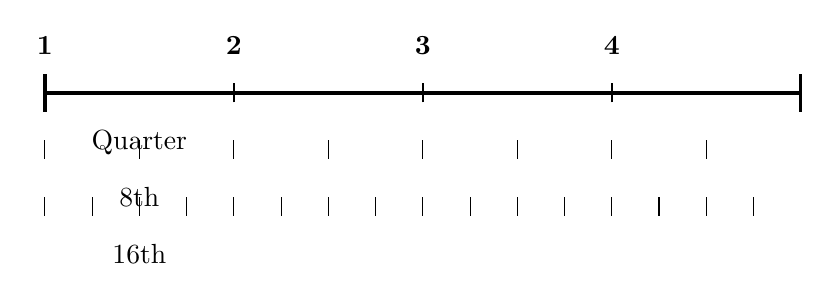
\begin{tikzpicture}[scale=1.2]
    % Draw the bar
    \draw[very thick] (0,0) -- (8,0);
    \draw[very thick] (0,-0.2) -- (0,0.2);
    \draw[very thick] (8,-0.2) -- (8,0.2);
    
    % Quarter notes
    \foreach \x in {0,2,4,6} {
        \draw[thick] (\x,-0.1) -- (\x,0.1);
    }
    \node[below] at (1,-0.3) {Quarter};
    
    % 8th notes
    \foreach \x in {0,1,2,3,4,5,6,7} {
        \draw (\x,-0.7) -- (\x,-0.5);
    }
    \node[below] at (1,-0.9) {8th};
    
    % 16th notes
    \foreach \x in {0,0.5,1,1.5,2,2.5,3,3.5,4,4.5,5,5.5,6,6.5,7,7.5} {
        \draw[thin] (\x,-1.3) -- (\x,-1.1);
    }
    \node[below] at (1,-1.5) {16th};
    
    % Beat numbers
    \node[above] at (0,0.3) {\textbf{1}};
    \node[above] at (2,0.3) {\textbf{2}};
    \node[above] at (4,0.3) {\textbf{3}};
    \node[above] at (6,0.3) {\textbf{4}};
\end{tikzpicture}

\textit{One bar divided into quarter notes, 8th notes, and 16th notes}
\end{center}

\textbf{\bluepurple{Why It Matters:}} Understanding note lengths helps you understand the grid in your DAW. When you see tiny divisions on the timeline, those are 16th or 32nd notes. The bigger divisions are quarter notes (beats) and bars.

\subsubsection{The Grid in Your DAW}

Your DAW (Digital Audio Workstation) has a \textbf{grid} that divides time into beats and subdivisions.

\textbf{\purple{What It Is:}} The vertical lines you see in your DAW's timeline—they show you where beats, 8th notes, and 16th notes fall.

Most DAWs let you change the grid resolution:
\begin{itemize}[leftmargin=*]
\item \textbf{1/4 note grid} - Snap to beats (1, 2, 3, 4)
\item \textbf{1/8 note grid} - Snap to 8th notes (half-beats)
\item \textbf{1/16 note grid} - Snap to 16th notes (common for precision)
\item \textbf{1/32 note grid} - Very fine detail
\end{itemize}

\textbf{\bluepurple{Why It Matters:}} The grid keeps your notes aligned and in-time. When you place a kick drum on the grid, it lands exactly on the beat. You can turn the grid off for more natural, loose timing, but starting with the grid helps you stay organized.

\textbf{\orangetext{Try It Yourself:}} 

In your DAW, look at the piano roll or drum editor. See those vertical lines? Those are the grid. Try these experiments:

\begin{enumerate}[leftmargin=*]
\item Set your grid to 1/4 notes and place kicks on beats 1 and 3
\item Change the grid to 1/8 notes and add hi-hats between the kicks
\item Change to 1/16 notes and create a fast hi-hat roll
\end{enumerate}

Watch how the grid helps you place notes exactly where you want them in time.

\subsubsection{Quantize}

\textbf{Quantization} is the process of snapping notes to the grid—making them perfectly on-time.

\textbf{\purple{What It Is:}} Taking notes you played (which might be slightly off-time) and moving them to the nearest grid position.

If you play a kick drum and it's slightly early or late, quantizing moves it to land exactly on beat 1.

\textbf{\bluepurple{Why It Matters:}} 
\begin{itemize}[leftmargin=*]
\item \textbf{Pro:} Makes your beats tight, clean, and professional-sounding
\item \textbf{Con:} Can make things sound too robotic if overused
\end{itemize}

\textbf{The balance:} Many producers quantize drums heavily but leave melodies and bass lines slightly loose for a more human feel.

\textbf{\greentext{In Real Songs:}} Modern hip-hop and EDM use heavy quantization for tight, punchy drums. Jazz, funk, and soul often use less quantization for a looser, more human groove.

\begin{tcolorbox}[colback=orange!10,colframe=orange,width=\textwidth,arc=3mm,boxrule=1pt]
\textbf{\orangetext{Try It Yourself:}}

\begin{enumerate}[leftmargin=*]
\item Play some drum hits without worrying about perfect timing
\item Select all the notes
\item Hit your DAW's quantize function (usually a button or Cmd+U / Ctrl+U)
\item Watch the notes snap to the grid—instant tightness!
\end{enumerate}

Experiment with quantize strength. Many DAWs let you quantize at 50\% or 75\%, keeping some human looseness while still cleaning up major timing issues.
\end{tcolorbox}

\vspace{1cm}

\begin{center}
\rule{0.8\textwidth}{0.5pt}

\vspace{0.3cm}

\textit{You now understand rhythm, beats, bars, and how time works in music. \\
Next up: Pitch—high notes, low notes, and everything in between.}

\vspace{0.3cm}

\rule{0.8\textwidth}{0.5pt}
\end{center}

\newpage

% ============================================================================
% PART 2: PITCH - HIGH AND LOW
% ============================================================================

\section{Part 2: Pitch — High and Low}

Now that you understand rhythm and time, let's explore the other fundamental element of music: \textbf{pitch}—how high or low sounds are. This is where notes, scales, melodies, and chords come from.

% ----------------------------------------------------------------------------
% CHAPTER 4: NOTES AND THE PIANO
% ----------------------------------------------------------------------------

\subsection{Chapter 4: Notes and the Piano}

\subsubsection{What is Pitch?}

\textbf{Pitch} is how high or low a sound is.

\textbf{\purple{What It Is:}} Pitch is determined by how fast something vibrates. Fast vibrations = high pitch. Slow vibrations = low pitch.

\begin{itemize}[leftmargin=*]
\item A bass drum vibrates slowly → low pitch
\item A hi-hat vibrates quickly → high pitch
\item A kick is lower than a snare, which is lower than a hi-hat
\end{itemize}

\textbf{\bluepurple{Why It Matters:}} Understanding pitch helps you create melodies, basslines, and chords. When you move notes "up" in your DAW's piano roll, you're increasing the pitch (making the vibration faster).

\subsubsection{Notes - The 12 Building Blocks}

Western music uses \textbf{12 different pitches} that repeat over and over:

\begin{center}
\textbf{C — C\# — D — D\# — E — F — F\# — G — G\# — A — A\# — B}

(then it repeats: C — C\# — D — D\#...)
\end{center}

\textbf{\purple{What It Is:}} These 12 notes are the alphabet of music. Just like English has 26 letters that combine to make words, music has 12 notes that combine to make melodies and chords.

Each note has a name:
\begin{itemize}[leftmargin=*]
\item \textbf{Natural notes:} C, D, E, F, G, A, B (the white keys on a piano)
\item \textbf{Sharp notes (\#):} C\#, D\#, F\#, G\#, A\# (the black keys)
\item \textbf{Flat notes (♭):} Same as sharps, just named differently (C\# = D♭)
\end{itemize}

The distance between each note is called a \textbf{semitone} or \textbf{half-step}. That's the smallest distance in Western music.

\textbf{\bluepurple{Why It Matters:}} Every melody, bassline, and chord you'll ever make uses these 12 notes. They're your raw materials.

\subsubsection{The Piano Keyboard - Your Visual Map}

The piano keyboard is the best way to visualize pitch. Even if you're not a piano player, understanding the keyboard layout is essential for modern production.

\begin{center}
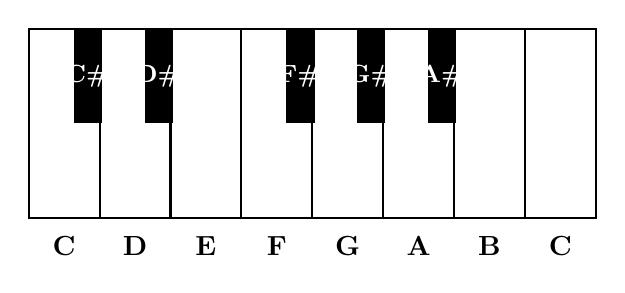
\begin{tikzpicture}[scale=0.6]
    % White keys
    \foreach \x in {0,1,2,3,4,5,6,7} {
        \draw[thick] (\x*1.5,0) rectangle (\x*1.5+1.5,4);
    }
    
    % Black keys
    \fill[black] (0.95,2) rectangle (1.55,4);
    \fill[black] (2.45,2) rectangle (3.05,4);
    % Skip E
    \fill[black] (5.45,2) rectangle (6.05,4);
    \fill[black] (6.95,2) rectangle (7.55,4);
    \fill[black] (8.45,2) rectangle (9.05,4);
    
    % Note labels on white keys
    \node[below] at (0.75,-0.2) {\textbf{C}};
    \node[below] at (2.25,-0.2) {\textbf{D}};
    \node[below] at (3.75,-0.2) {\textbf{E}};
    \node[below] at (5.25,-0.2) {\textbf{F}};
    \node[below] at (6.75,-0.2) {\textbf{G}};
    \node[below] at (8.25,-0.2) {\textbf{A}};
    \node[below] at (9.75,-0.2) {\textbf{B}};
    \node[below] at (11.25,-0.2) {\textbf{C}};
    
    % Note labels on black keys
    \node[white] at (1.25,3) {\small\textbf{C\#}};
    \node[white] at (2.75,3) {\small\textbf{D\#}};
    \node[white] at (5.75,3) {\small\textbf{F\#}};
    \node[white] at (7.25,3) {\small\textbf{G\#}};
    \node[white] at (8.75,3) {\small\textbf{A\#}};
\end{tikzpicture}

\textit{One octave on the piano keyboard}
\end{center}

\textbf{Notice the pattern:}
\begin{itemize}[leftmargin=*]
\item White keys are the natural notes (C, D, E, F, G, A, B)
\item Black keys are the sharps/flats (C\#, D\#, F\#, G\#, A\#)
\item The pattern of black keys: \textbf{two blacks, gap, three blacks, gap, repeat}
\end{itemize}

This pattern repeats up and down the entire keyboard. Once you recognize it, you can always find any note.

\textbf{Finding C:} C is always to the LEFT of the group of two black keys. This is your landmark note—always use C to orient yourself on the keyboard.

\textbf{\orangetext{Try It Yourself:}} 

Open your DAW's piano roll. See how it looks like a keyboard turned sideways? 

\begin{itemize}[leftmargin=*]
\item Find a C note (left of the two-black-key group)
\item Count up: C → D → E → F → G → A → B → C
\item Play those notes—you just played a C major scale!
\end{itemize}

\subsubsection{Octaves}

An \textbf{octave} is the distance from one note to the next note with the same name.

\textbf{\purple{What It Is:}} The same note, just higher or lower. C2 is a low C. C4 is middle C. C6 is a high C. They're all "C," just in different ranges.

\textbf{\bluepurple{Why It Matters:}} 
\begin{itemize}[leftmargin=*]
\item \textbf{Bass notes} live in the low octaves (C2, C3)
\item \textbf{Chords} usually sit in the middle octaves (C3, C4, C5)
\item \textbf{Melodies} often sit in higher octaves (C5, C6)
\end{itemize}

When you move a note up or down an octave, it keeps the same character but changes range. A C is always a C, whether it's low or high.

\textbf{\greentext{In Real Songs:}}
\begin{itemize}[leftmargin=*]
\item "Come Together" - The bass plays D in a low octave (D2)
\item "Still D.R.E." - The piano riff plays C and A in the middle range (C4-A3)
\item Most kick drums are tuned around C1 or C2 (very low)
\end{itemize}

\begin{tcolorbox}[colback=lightgray,colframe=purple,width=\textwidth,arc=3mm,boxrule=1pt]
\textbf{Octave Numbering:}

MIDI uses octave numbers to tell notes apart:
\begin{itemize}[leftmargin=*]
\item \textbf{C1, C2} - Very low (bass, kick drums)
\item \textbf{C3, C4} - Middle range (chords, mid-range melodies)
\item \textbf{C5, C6} - High range (lead melodies, high synths)
\item \textbf{C7, C8} - Very high (top of the range)
\end{itemize}

Different DAWs sometimes number octaves differently (some call middle C "C3," others call it "C4"). Don't stress about it—the concept is the same.
\end{tcolorbox}

\textbf{\orangetext{Try It Yourself:}}

In your piano roll:
\begin{enumerate}[leftmargin=*]
\item Place a note on C3
\item Copy it to C4 (one octave higher)
\item Copy it to C2 (one octave lower)
\item Play them in sequence—same note, different heights!
\end{enumerate}

\newpage

% ----------------------------------------------------------------------------
% CHAPTER 5: SCALES - CHOOSING YOUR NOTES
% ----------------------------------------------------------------------------

\subsection{Chapter 5: Scales — Choosing Your Notes}

You now know there are 12 notes available. But if you use all 12 at once, it sounds chaotic. A \textbf{scale} is a selection of notes that sound good together.

\subsubsection{What is a Scale?}

\textbf{\purple{What It Is:}} A scale is a set of notes chosen from the 12 available notes. Instead of using all 12, you pick 5, 7, or 8 notes that work well together.

Think of it like a color palette. You have every color available, but when painting, you choose a specific palette that creates harmony.

\textbf{\bluepurple{Why It Matters:}} Scales give you a framework. When you stick to the notes in a scale, everything you play will sound musical and cohesive. You can't really play a "wrong" note if you stay in your scale.

\subsubsection{Major Scale - The Happy Scale}

The \textbf{major scale} is the foundation of Western music. It has 7 notes and sounds bright, happy, and uplifting.

\textbf{\purple{What It Is:}} A specific pattern of whole steps and half steps that creates a happy, bright sound.

\textbf{C Major Scale:} C — D — E — F — G — A — B — (C)

This is the famous "Do-Re-Mi-Fa-Sol-La-Ti-Do" you might have heard.

\begin{tcolorbox}[colback=lightgray,colframe=green,width=\textwidth,arc=3mm,boxrule=1pt]
\textbf{C Major is the Easiest:}

C Major uses only the white keys on the piano—no black keys (no sharps or flats). This makes it the easiest scale to visualize and play. Start on C, play only white keys, stop at the next C. That's C Major.
\end{tcolorbox}

\textbf{\greentext{In Real Songs:}}
\begin{itemize}[leftmargin=*]
\item "Levels" by Avicii - E Major (bright, euphoric EDM)
\item Most pop songs use major scales for choruses (uplifting energy)
\item Happy birthday, nursery rhymes—almost all major scale
\end{itemize}

\textbf{\orangetext{Try It Yourself:}}

In your piano roll, starting from C4, place notes on: C, D, E, F, G, A, B, C (only white keys). Play them in order. That's the major scale—the sound of happiness and brightness.

\subsubsection{Minor Scale - The Emotional Scale}

The \textbf{minor scale} is darker, more emotional, and more introspective than major.

\textbf{\purple{What It Is:}} A scale with a lowered 3rd note compared to major, creating a sadder, darker sound.

\textbf{A Minor Scale:} A — B — C — D — E — F — G — (A)

Notice: A Minor has the exact same notes as C Major, just starting from a different note. This is called the "relative minor."

\begin{tcolorbox}[colback=lightgray,colframe=blue,width=\textwidth,arc=3mm,boxrule=1pt]
\textbf{A Minor is Also All White Keys:}

Like C Major, A Minor uses only white keys. Start on A, play white keys to the next A. This is your natural minor scale. Simple and beautiful.
\end{tcolorbox}

\textbf{\greentext{In Real Songs:}}
\begin{itemize}[leftmargin=*]
\item "Still D.R.E." - E Minor / A Minor (dark, hypnotic G-Funk)
\item "Come Together" - D Minor (swampy, bluesy vibe)
\item Hip-hop, trap, and emotional pop often use minor scales
\end{itemize}

\textbf{\bluepurple{Why It Matters:}} 

Major vs. Minor is one of the biggest decisions in your beat. Want it happy and uplifting? Major. Want it dark, emotional, or moody? Minor. This single choice sets the entire emotional tone.

\textbf{\orangetext{Try It Yourself:}}

Play your C Major scale again (C-D-E-F-G-A-B-C). Now play A Minor (A-B-C-D-E-F-G-A). Same notes, different starting point, completely different feeling. The major sounds bright; the minor sounds introspective.

\subsubsection{Pentatonic Scale - The Beatmaker's Best Friend}

The \textbf{pentatonic scale} uses only 5 notes (penta = five). It's incredibly forgiving—you can play almost any combination and it sounds good.

\textbf{\purple{What It Is:}} A 5-note scale that removes the "tension" notes, leaving only notes that sound good together.

\textbf{C Major Pentatonic:} C — D — E — G — A

\textbf{A Minor Pentatonic:} A — C — D — E — G

Notice: No F or B. Those are the notes that can sound "wrong" if used carelessly. By removing them, you get a scale where you literally can't hit a bad note.

\textbf{\bluepurple{Why It Matters:}} The pentatonic scale is perfect for improvising, creating melodies, and jamming. It's used extensively in blues, rock, hip-hop, and EDM.

Many legendary guitar solos, piano riffs, and hip-hop melodies use pentatonic scales because they're so reliable and musical.

\textbf{\greentext{In Real Songs:}}
\begin{itemize}[leftmargin=*]
\item Most blues guitar solos - pentatonic scale
\item "My Girl" by The Temptations - pentatonic bass line
\item Countless hip-hop beats use minor pentatonic for melodies
\end{itemize}

\textbf{\orangetext{Try It Yourself:}}

In your piano roll, place notes on the black keys only: C\#, D\#, F\#, G\#, A\#. 

Play any combination of these notes in any order. Notice how everything sounds good together? That's the magic of the pentatonic scale. You can randomly hit black keys and it'll sound musical.

\vspace{1cm}

\begin{center}
\rule{0.6\textwidth}{0.5pt}

\vspace{0.3cm}

\textit{Pro Tip: Start with pentatonic when creating melodies. \\
Once you're comfortable, expand to the full major or minor scale.}

\vspace{0.3cm}

\rule{0.6\textwidth}{0.5pt}
\end{center}

\newpage

% ----------------------------------------------------------------------------
% CHAPTER 6: KEY - THE HOME BASE
% ----------------------------------------------------------------------------

\subsection{Chapter 6: Key — The Home Base}

Now that you understand scales, let's talk about \textbf{key}—which scale your entire song is using.

\subsubsection{What is a Key?}

\textbf{\purple{What It Is:}} The key tells you which scale and which starting note your song is built around.

When someone says "this song is in C Major," they mean:
\begin{itemize}[leftmargin=*]
\item It uses the notes from the C Major scale
\item C feels like "home"—the most stable, resolved note
\item Most melodies, chords, and bass lines use notes from C Major
\end{itemize}

\textbf{\bluepurple{Why It Matters:}} The key unifies your entire track. Your drums can be any pitch, but your bass, chords, and melody should all use notes from the same key. This creates harmonic consistency.

\subsubsection{Major Keys vs. Minor Keys}

Every key comes in two flavors:

\textbf{Major Keys} - Bright, happy, uplifting
\begin{itemize}[leftmargin=*]
\item C Major, E Major, G Major, etc.
\item Common in pop, EDM, dance music
\item "Levels" by Avicii - E Major
\end{itemize}

\textbf{Minor Keys} - Dark, emotional, introspective
\begin{itemize}[leftmargin=*]
\item A Minor, E Minor, D Minor, etc.
\item Common in hip-hop, trap, emotional music
\item "Still D.R.E." - A Minor / E Minor
\item "Come Together" - D Minor
\end{itemize}

\subsubsection{The Tonal Center - Finding Home}

The \textbf{tonal center} is the note that feels like "home"—the most stable and resolved.

\textbf{\purple{What It Is:}} The note that your melody wants to return to. When you end on the tonal center, it feels complete and resolved. When you end on other notes, it feels unresolved or tense.

If your song is in C Major, C is the tonal center. Play the C Major scale and stop on B—it feels incomplete, like it needs one more note. Now play it again and stop on C—it feels finished.

\textbf{\bluepurple{Why It Matters:}} Understanding the tonal center helps you create resolution and tension. Ending phrases on the tonal center feels resolved. Ending on other notes creates tension or leaves the listener wanting more.

\subsubsection{Staying in Key}

\textbf{Staying in key} means using only notes from your chosen scale.

If you're in C Major:
\begin{itemize}[leftmargin=*]
\item Your bass line should use notes from C Major
\item Your chords should be built from C Major notes
\item Your melody should use C Major notes
\end{itemize}

\textbf{\greentext{In Real Songs:}} Most pop, rock, hip-hop, and EDM stay in one key for the entire song. This creates consistency and makes everything sound cohesive.

Some advanced songs change keys (called \textbf{modulation}), but that's not something to worry about as a beginner.

\begin{tcolorbox}[colback=orange!10,colframe=orange,width=\textwidth,arc=3mm,boxrule=1pt]
\textbf{\orangetext{Try It Yourself:}}

\begin{enumerate}[leftmargin=*]
\item Pick a key (start with C Major or A Minor)
\item Create a bass line using only those scale notes
\item Add a melody using only those scale notes
\item Add chords using only those scale notes
\end{enumerate}

Everything will sound harmonically connected because you stayed in key.
\end{tcolorbox}

\subsubsection{Why Keys Matter for Production}

\textbf{Collaboration \& Layering:}
\begin{itemize}[leftmargin=*]
\item If your bass is in A Minor, your chords should be too
\item If you add a sample or vocal, check what key it's in
\item Layering sounds in different keys creates dissonance (clash)
\end{itemize}

\textbf{Choosing Your Key:}

Most DAWs default to C Major. But you can choose any key. Here's how to decide:

\begin{itemize}[leftmargin=*]
\item \textbf{Mood:} Major for happy, Minor for dark
\item \textbf{Vocal range:} Singers have comfortable ranges
\item \textbf{Genre trends:} Hip-hop often uses minor keys; pop uses both
\item \textbf{Sound design:} Lower keys (like E Minor or D Minor) sound heavier and darker
\end{itemize}

\begin{center}
\rule{0.6\textwidth}{0.5pt}

\vspace{0.3cm}

\textit{You now understand rhythm, pitch, scales, and keys—the foundation! \\
Next: How notes work together through intervals, chords, and progressions.}

\vspace{0.3cm}

\rule{0.6\textwidth}{0.5pt}
\end{center}

% ============================================================================
% PART 3: HARMONY - NOTES TOGETHER
% ============================================================================

\section{Part 3: Harmony — Notes Together}

You've learned about individual notes, scales, and keys. Now let's explore what happens when you play notes \textit{together}—creating harmony through intervals, chords, and progressions.

% ----------------------------------------------------------------------------
% CHAPTER 7: INTERVALS - DISTANCE BETWEEN NOTES
% ----------------------------------------------------------------------------

\subsection{Chapter 7: Intervals — Distance Between Notes}

An \textbf{interval} is the distance between two notes. Intervals are the building blocks of melodies and chords.

\subsubsection{What is an Interval?}

\textbf{\purple{What It Is:}} The gap between two notes, measured in steps. Intervals can be small (two adjacent notes) or large (notes far apart).

Think of intervals like distances: the distance from your house to the corner store (small interval) vs. the distance to the next city (large interval).

\textbf{\bluepurple{Why It Matters:}} Different intervals create different feelings:
\begin{itemize}[leftmargin=*]
\item Small intervals = smooth, melodic
\item Large intervals = dramatic, powerful
\item Certain intervals sound tense, others sound resolved
\end{itemize}

\subsubsection{Common Intervals Every Beatmaker Should Know}

\textbf{1. Unison} - Same note (0 semitones)
\begin{itemize}[leftmargin=*]
\item Playing C and C together
\item Doubling—when two instruments play the same note
\end{itemize}

\textbf{2. Octave} - 12 semitones
\begin{itemize}[leftmargin=*]
\item C to the next C (higher or lower)
\item Sounds like the same note, just different height
\item Very consonant (pleasant, stable)
\end{itemize}

\textbf{3. Perfect 5th} - 7 semitones
\begin{itemize}[leftmargin=*]
\item C to G, A to E
\item Powerful, open, strong sound
\item The foundation of power chords in rock
\item Used heavily in "Still D.R.E." (A to E)
\end{itemize}

\textbf{4. Major 3rd} - 4 semitones
\begin{itemize}[leftmargin=*]
\item C to E, G to B
\item Sweet, happy, pleasant
\item Makes major chords sound "major"
\end{itemize}

\textbf{5. Minor 3rd} - 3 semitones
\begin{itemize}[leftmargin=*]
\item A to C, E to G
\item Darker, sadder, more introspective
\item Makes minor chords sound "minor"
\end{itemize}

\textbf{\greentext{In Real Songs:}}
\begin{itemize}[leftmargin=*]
\item "Still D.R.E." - Perfect 5th (A to E) in the bass creates power
\item "Levels" - Major 3rds in the melody create brightness
\item Power chords in rock - Root note + Perfect 5th
\end{itemize}

\textbf{\orangetext{Try It Yourself:}}

In your piano roll:
\begin{enumerate}[leftmargin=*]
\item Play C and G together (Perfect 5th) - sounds powerful and open
\item Play C and E together (Major 3rd) - sounds sweet and happy
\item Play C and E♭ together (Minor 3rd) - sounds darker and sadder
\end{enumerate}

Feel how different intervals create different emotions.

\newpage

% ----------------------------------------------------------------------------
% CHAPTER 8: CHORDS - MULTIPLE NOTES AT ONCE
% ----------------------------------------------------------------------------

\subsection{Chapter 8: Chords — Multiple Notes at Once}

A \textbf{chord} is three or more notes played together. Chords create the harmonic foundation of your beat.

\subsubsection{What is a Chord?}

\textbf{\purple{What It Is:}} Multiple notes stacked together to create harmony. Chords provide the "bed" that melodies sit on top of.

Think of chords like the stage or platform. Your melody is the performer, and the chords are the stage they perform on. The chords set the mood and support the melody.

\textbf{\bluepurple{Why It Matters:}} Chords create the emotional vibe of your track. Major chords feel happy. Minor chords feel sad. Different chord progressions create different emotional journeys.

\subsubsection{Triads - The Basic Chord}

A \textbf{triad} is the simplest chord: 3 notes stacked in 3rds.

\textbf{Building a Triad:}
\begin{enumerate}[leftmargin=*]
\item Start with the \textbf{root} (the main note)
\item Add the \textbf{3rd} (either major 3rd or minor 3rd)
\item Add the \textbf{5th} (usually a perfect 5th above the root)
\end{enumerate}

\textbf{Major Triad} - Root + Major 3rd + Perfect 5th
\begin{itemize}[leftmargin=*]
\item \textbf{C Major:} C — E — G (happy, bright)
\item \textbf{E Major:} E — G\# — B (uplifting)
\item \textbf{G Major:} G — B — D (cheerful)
\end{itemize}

\textbf{Minor Triad} - Root + Minor 3rd + Perfect 5th
\begin{itemize}[leftmargin=*]
\item \textbf{A Minor:} A — C — E (sad, introspective)
\item \textbf{E Minor:} E — G — B (dark, emotional)
\item \textbf{D Minor:} D — F — A (somber)
\end{itemize}

The only difference between major and minor is the 3rd—major 3rd = happy, minor 3rd = sad.

\textbf{\greentext{In Real Songs:}}
\begin{itemize}[leftmargin=*]
\item "Levels" - Uses major triads (E, B, A, C\#m) for that uplifting EDM feel
\item "Come Together" - Doesn't use full chords; stays minimal (vamp-based)
\item Most pop songs - Built on triads and extended chords
\end{itemize}

\subsubsection{Dyads - The Minimalist Approach}

A \textbf{dyad} is just 2 notes played together. It's simpler than a chord but can be just as powerful.

\textbf{\purple{What It Is:}} Two notes—often a root and a 5th, or a root and a 3rd.

\textbf{\bluepurple{Why It Matters:}} Dyads are minimal and leave space in the mix. They're perfect for modern production where you want clean, uncluttered harmony.

\textbf{\greentext{In Real Songs:}}
\begin{itemize}[leftmargin=*]
\item \textbf{"Still D.R.E."} - The piano riff is literally just a dyad: C and A played together
\item Power chords in rock/metal - Root + 5th (like C + G)
\item Modern trap and hip-hop often use dyads instead of full chords
\end{itemize}

\textbf{\orangetext{Try It Yourself:}}

\begin{enumerate}[leftmargin=*]
\item Build a C Major triad: C, E, G (play them together)
\item Build an A Minor triad: A, C, E (play them together)
\item Compare: major sounds happy, minor sounds sad
\item Now try a dyad: just C and A together—simple but effective
\end{enumerate}

\subsubsection{Extended Chords}

Once you're comfortable with triads, you can add more notes to create richer, jazzier sounds:

\textbf{7th Chords} - Add a 7th note above the root
\begin{itemize}[leftmargin=*]
\item Cmaj7: C — E — G — B (jazzy, sophisticated)
\item Am7: A — C — E — G (smooth, soulful)
\item Dominant 7: C — E — G — B♭ (tense, wants to resolve)
\end{itemize}

\textbf{9th, 11th, 13th Chords} - Even more extended
\begin{itemize}[leftmargin=*]
\item Used in jazz, neo-soul, R\&B
\item Add color and complexity
\item Not essential for beginners—stick to triads first
\end{itemize}

\begin{tcolorbox}[colback=lightgray,colframe=purple,width=\textwidth,arc=3mm,boxrule=1pt]
\textbf{Beginner Focus:}

Start with major and minor triads. Master those before moving to 7ths and beyond. Most hit songs use simple triads—complexity isn't always better.
\end{tcolorbox}

\newpage

% ----------------------------------------------------------------------------
% CHAPTER 9: CHORD PROGRESSIONS - MOVEMENT
% ----------------------------------------------------------------------------

\subsection{Chapter 9: Chord Progressions — Movement}

A \textbf{chord progression} is a sequence of chords that creates harmonic movement and emotional journey.

\subsubsection{What is a Chord Progression?}

\textbf{\purple{What It Is:}} A series of chords played in order, usually repeating throughout a song or section.

Instead of staying on one chord, you move from chord to chord, creating tension and resolution, movement and flow.

\textbf{\bluepurple{Why It Matters:}} Chord progressions are the harmonic backbone of your song. They create the emotional arc and give your melody somewhere to go.

\subsubsection{Roman Numeral Analysis}

Musicians use Roman numerals to describe chord progressions relative to the key.

In C Major:
\begin{itemize}[leftmargin=*]
\item \textbf{I} = C Major (the tonic, "home")
\item \textbf{ii} = D Minor
\item \textbf{iii} = E Minor
\item \textbf{IV} = F Major (stable, resolved)
\item \textbf{V} = G Major (tension, wants to go back to I)
\item \textbf{vi} = A Minor (emotional, introspective)
\item \textbf{vii°} = B Diminished (rarely used)
\end{itemize}

\textbf{Capital} = Major chord. \textbf{Lowercase} = Minor chord.

\textbf{\bluepurple{Why It Matters:}} Using Roman numerals, you can transpose progressions to any key. A I-V-vi-IV progression works in C Major (C-G-Am-F) or in E Major (E-B-C\#m-A).

\subsubsection{Famous Chord Progressions}

\textbf{1. I-V-vi-IV (Pop Progression)}

The most common progression in modern pop, rock, and EDM.

\textbf{In C Major:} C — G — Am — F

\textbf{In E Major:} E — B — C\#m — A (used in "Levels" by Avicii)

\textbf{\greentext{Why It Works:}} Starts on home (I), moves to tension (V), drops to emotional (vi), then resolves back through (IV) to repeat. It's an emotional rollercoaster that feels complete.

\textbf{Songs Using This:}
\begin{itemize}[leftmargin=*]
\item "Let It Be" - The Beatles
\item "Don't Stop Believin'" - Journey
\item "Someone Like You" - Adele
\item "Levels" - Avicii
\item Thousands of pop hits
\end{itemize}

\vspace{0.5cm}

\textbf{2. i-iv (Minor Vamp)}

Two minor chords alternating—simple but hypnotic.

\textbf{In A Minor:} Am — Dm (or Am — Em)

\textbf{In E Minor:} Em — Am (used in "Still D.R.E.")

\textbf{\greentext{Why It Works:}} Minimal, hypnotic, and dark. Leaves tons of space for the beat and bass to shine. Common in hip-hop and G-Funk.

\textbf{Songs Using This:}
\begin{itemize}[leftmargin=*]
\item "Still D.R.E." - Dr. Dre
\item Many trap and hip-hop beats
\item Minimalist vamps
\end{itemize}

\vspace{0.5cm}

\textbf{3. One-Chord Vamp}

Not a progression at all—just one chord (or note) repeated.

\textbf{\greentext{Why It Works:}} Creates groove through rhythm rather than harmony. The interest comes from the drums, bass movement, and melody—not chord changes.

\textbf{Songs Using This:}
\begin{itemize}[leftmargin=*]
\item "Come Together" - The Beatles (D Minor vamp)
\item "Chameleon" - Herbie Hancock
\item Lots of funk and groove-based music
\end{itemize}

\vspace{0.5cm}

\textbf{4. I-IV-V (Blues/Rock Progression)}

The foundation of blues, rock and roll, and early rock music.

\textbf{In C Major:} C — F — G

\textbf{\greentext{Why It Works:}} These three chords form the backbone of Western music. Simple, direct, powerful.

\textbf{Songs Using This:}
\begin{itemize}[leftmargin=*]
\item "Twist and Shout" - The Beatles
\item "La Bamba" - Ritchie Valens
\item Countless blues and rock songs
\end{itemize}

\subsubsection{Creating Your Own Progressions}

Start simple:

\begin{enumerate}[leftmargin=*]
\item \textbf{Pick your key} (C Major or A Minor are easiest)
\item \textbf{Start on I (or i)} - the home chord
\item \textbf{Move to IV or V} - stable or tense
\item \textbf{Try vi} - for emotional depth
\item \textbf{Loop back to I} - return home
\end{enumerate}

Experiment with different orders. Not every progression needs to be I-V-vi-IV. Try:
\begin{itemize}[leftmargin=*]
\item vi-IV-I-V (starts emotional)
\item I-vi-IV-V (similar to pop progression)
\item i-VII-VI-V (minor progression with descending bass)
\end{itemize}

\textbf{\orangetext{Try It Yourself:}}

\begin{enumerate}[leftmargin=*]
\item Open your DAW and set it to 90 BPM
\item Create a chord track in C Major
\item Build the I-V-vi-IV progression: C, G, Am, F
\item Hold each chord for 4 beats (one bar each)
\item Loop it and listen—this is the sound of pop music
\item Now try Am, F, C, G (vi-IV-I-V) - different vibe, same chords
\end{enumerate}

\begin{center}
\rule{0.6\textwidth}{0.5pt}

\vspace{0.3cm}

\textit{You now understand harmony! Intervals, chords, and progressions \\
are the tools you use to create emotional movement in your music.}

\vspace{0.3cm}

\rule{0.6\textwidth}{0.5pt}
\end{center}

\newpage

% ============================================================================
% PART 4: BEATMAKER'S TOOLKIT
% ============================================================================

\section*{PART 4: THE BEATMAKER'S TOOLKIT}

Now you know the fundamentals: rhythm, pitch, and harmony. Let's talk about the actual sounds you'll work with—the instruments that make up a beat.

\subsection{Chapter 10: Drums — The Foundation}

Drums are the backbone of almost every beat. They provide rhythm, energy, and structure.

\subsubsection{What Makes Up a Drum Kit?}

A standard drum kit has several key pieces. In production, you'll often program these sounds individually in your DAW.

\vspace{0.5cm}

\textbf{1. Kick Drum (Bass Drum)}

\textbf{\purple{What It Is:}} The lowest, deepest drum sound—a big "BOOM." 

\textbf{\bluepurple{Where It Hits:}} Typically on beats 1 and 3 in a 4/4 pattern ("1-2-3-4"). Often called "four-on-the-floor" in dance music when it hits all four beats.

\textbf{\greentext{Why It Matters:}} The kick drum drives the low end and gives your beat weight. It's the foundation everything else sits on.

\textbf{Common Patterns:}
\begin{itemize}[leftmargin=*]
\item \textbf{Four-on-the-floor:} Kick on every beat (1-2-3-4) — House, techno, EDM
\item \textbf{1 \& 3:} Kick on beats 1 and 3 — Rock, pop
\item \textbf{Syncopated:} Kicks between the beats — Hip-hop, trap, funk
\end{itemize}

\vspace{0.5cm}

\textbf{2. Snare Drum}

\textbf{\purple{What It Is:}} A sharp, cracking drum sound with wires (called "snares") stretched across the bottom. Sounds like "CRACK" or "POP."

\textbf{\bluepurple{Where It Hits:}} Typically on beats 2 and 4—called the \textbf{backbeat}.

\textbf{\greentext{Why It Matters:}} The snare creates the rhythmic tension against the kick. When you clap along to a song, you're usually clapping on the snare (beats 2 and 4).

\textbf{Common Patterns:}
\begin{itemize}[leftmargin=*]
\item \textbf{Backbeat:} Snare on 2 and 4 — Nearly universal in Western music
\item \textbf{Syncopated snares:} Adding extra hits between 2 and 4 — Hip-hop, trap
\item \textbf{Rolls:} Rapid snare hits for fills and transitions
\end{itemize}

\vspace{0.5cm}

\textbf{3. Hi-Hat}

\textbf{\purple{What It Is:}} Two small cymbals that crash together, creating a "tss-tss-tss" sound.

\textbf{\bluepurple{Types:}}
\begin{itemize}[leftmargin=*]
\item \textbf{Closed hi-hat:} Tight, short "tss" — most common
\item \textbf{Open hi-hat:} Longer, ringing "tssshhh" — for accents
\end{itemize}

\textbf{\greentext{Why It Matters:}} Hi-hats create the rhythmic texture and drive the groove. They're often the most frequent sound in a drum pattern.

\textbf{Common Patterns:}
\begin{itemize}[leftmargin=*]
\item \textbf{8th notes:} "tss-tss-tss-tss-tss-tss-tss-tss" (8 hits per bar) — Rock, pop
\item \textbf{16th notes:} Double-time for faster, busier patterns — Hip-hop, trap
\item \textbf{Triplets:} Three hits per beat for swing/shuffle feel — Jazz, blues
\end{itemize}

\vspace{0.5cm}

\textbf{4. Cymbals (Crash, Ride)}

\textbf{\purple{What They Are:}} Large, ringing metal discs.

\textbf{\bluepurple{Types:}}
\begin{itemize}[leftmargin=*]
\item \textbf{Crash:} Big, explosive "CRASH" for emphasis and transitions
\item \textbf{Ride:} Sustained "ping-ping-ping" used instead of hi-hats for different texture
\end{itemize}

\textbf{\greentext{Why They Matter:}} Crashes mark important moments—the start of a chorus, the peak of a buildup. Rides provide alternative rhythmic texture.

\vspace{0.5cm}

\textbf{5. Toms}

\textbf{\purple{What They Are:}} Cylindrical drums of various sizes, creating pitched drum tones.

\textbf{\bluepurple{Types:}}
\begin{itemize}[leftmargin=*]
\item \textbf{High tom:} Higher-pitched "doo"
\item \textbf{Mid tom:} Medium "boom"
\item \textbf{Floor tom:} Low, resonant "BOOM"
\end{itemize}

\textbf{\greentext{Why They Matter:}} Toms are used for fills—transitional drum phrases that lead from one section to another.

\vspace{0.5cm}

\textbf{6. Percussion}

\textbf{\purple{What It Is:}} Additional rhythm instruments beyond the core kit.

\textbf{Common Percussion Sounds:}
\begin{itemize}[leftmargin=*]
\item \textbf{Shakers:} "shh-shh-shh" texture
\item \textbf{Tambourine:} Jingly accent hits
\item \textbf{Cowbell:} Metallic "dink-dink"
\item \textbf{Congas/Bongos:} Pitched hand drums
\item \textbf{Claps:} Hand clap sound, often instead of or layered with snare
\end{itemize}

\textbf{\greentext{Why It Matters:}} Percussion adds character, texture, and rhythmic interest beyond the basic drum kit.

\subsubsection{Basic Drum Patterns}

Let's look at some fundamental patterns:

\vspace{0.5cm}

\textbf{Pattern 1: Basic 4/4 Rock/Pop Beat}

\begin{center}
\begin{tabular}{l l l l l l l l l}
Beat: & 1 & + & 2 & + & 3 & + & 4 & + \\
\hline
Kick: & \textbf{X} & & & & \textbf{X} & & & \\
Snare: & & & \textbf{X} & & & & \textbf{X} & \\
Hi-Hat: & \textbf{X} & \textbf{X} & \textbf{X} & \textbf{X} & \textbf{X} & \textbf{X} & \textbf{X} & \textbf{X} \\
\end{tabular}
\end{center}

\begin{itemize}[leftmargin=*]
\item Kick on 1 and 3
\item Snare on 2 and 4 (backbeat)
\item Hi-hat on every 8th note
\end{itemize}

This is the most fundamental drum pattern in modern music. Learn this first.

\vspace{0.5cm}

\textbf{Pattern 2: Four-on-the-Floor (House/EDM)}

\begin{center}
\begin{tabular}{l l l l l l l l l}
Beat: & 1 & + & 2 & + & 3 & + & 4 & + \\
\hline
Kick: & \textbf{X} & & \textbf{X} & & \textbf{X} & & \textbf{X} & \\
Snare: & & & \textbf{X} & & & & \textbf{X} & \\
Hi-Hat: & \textbf{X} & \textbf{X} & \textbf{X} & \textbf{X} & \textbf{X} & \textbf{X} & \textbf{X} & \textbf{X} \\
\end{tabular}
\end{center}

\begin{itemize}[leftmargin=*]
\item Kick on every beat (1-2-3-4)
\item Snare still on 2 and 4
\item Hi-hat on every 8th note
\end{itemize}

This is the foundation of house, techno, and most dance music.

\vspace{0.5cm}

\textbf{Pattern 3: Hip-Hop Boom-Bap}

\begin{center}
\begin{tabular}{l l l l l l l l l}
Beat: & 1 & + & 2 & + & 3 & + & 4 & + \\
\hline
Kick: & \textbf{X} & & & & & & \textbf{X} & \\
Snare: & & & \textbf{X} & & & & \textbf{X} & \\
Hi-Hat: & \textbf{X} & \textbf{x} & \textbf{X} & \textbf{x} & \textbf{X} & \textbf{x} & \textbf{X} & \textbf{x} \\
\end{tabular}
\end{center}

(Capital X = loud hit, lowercase x = soft hit for hi-hat)

\begin{itemize}[leftmargin=*]
\item Kick on 1 and the "+" after beat 3
\item Snare on 2 and 4
\item Hi-hat on 8th notes with alternating velocities (loud/soft pattern)
\end{itemize}

Classic hip-hop groove.

\textbf{\orangetext{Try It Yourself:}}

\begin{enumerate}[leftmargin=*]
\item Open your DAW and create a MIDI track with a drum kit plugin
\item Set your tempo to 90 BPM
\item Program Pattern 1 (Basic 4/4 Rock Beat)
\item Listen to it loop—this is the foundation of a beat
\item Now try Pattern 2 (Four-on-the-Floor) at 125 BPM—feel how it changes the energy
\end{enumerate}

\newpage

\subsection{Chapter 11: Bass — The Low End}

Bass is the low-pitched foundation that sits between the drums and the melodic elements.

\subsubsection{What is Bass?}

\textbf{\purple{Definition:}} Bass refers to the lowest melodic notes in your track. Bass plays notes (not just rhythm like drums) but focuses on the low frequencies you feel as much as hear.

\textbf{\bluepurple{Frequency Range:}} Roughly 40-250 Hz (the rumble and boom you feel in your chest).

\textbf{\greentext{Why It Matters:}} Bass glues the drums to the harmony. It provides weight, groove, and often defines the chord changes.

\subsubsection{Types of Bass Sounds}

\textbf{1. Bass Guitar}

\textbf{\purple{What It Is:}} A 4-string guitar tuned an octave lower than a regular guitar. The classic organic bass sound.

\textbf{Used In:} Rock, funk, soul, R\&B, jazz, pop

\textbf{Sound Character:} Warm, round, plucky. Think Motown, funk, classic rock.

\textbf{Famous Example:} "Come Together" by The Beatles

\vspace{0.5cm}

\textbf{2. Synth Bass}

\textbf{\purple{What It Is:}} Bass sounds created by synthesizers—from smooth sine wave subs to aggressive sawtooth growls.

\textbf{Used In:} Hip-hop, EDM, trap, pop, R\&B

\textbf{Sound Character:} Can be anything—deep and smooth, aggressive and distorted, or bouncy and plucky.

\textbf{Famous Example:} "Still D.R.E." by Dr. Dre (smooth synth bass)

\vspace{0.5cm}

\textbf{3. 808 Bass}

\textbf{\purple{What It Is:}} A specific bass drum sound from the Roland TR-808 drum machine, now used as a pitched bass sound. Deep, booming, and sustained.

\textbf{Used In:} Hip-hop, trap, modern R\&B

\textbf{Sound Character:} Deep sub-bass rumble with a pitch. Feels more than heard on small speakers.

\textbf{Famous Example:} Nearly every modern trap and hip-hop song

\vspace{0.5cm}

\textbf{4. Sub-Bass}

\textbf{\purple{What It Is:}} Pure low-frequency sine wave (20-60 Hz). You feel it more than hear it.

\textbf{Used In:} EDM, dubstep, hip-hop, trap

\textbf{Sound Character:} Pure rumble. No harmonics, just deep fundamental frequency.

\textbf{Famous Example:} The "drop" in dubstep and bass music

\subsubsection{What Does Bass Do?}

Bass has three main jobs:

\textbf{1. Lock with the Drums}

The bass and kick drum work together to create a unified low-end groove. When the kick hits, the bass often plays at the same time, reinforcing the rhythm.

\textbf{2. Define the Harmony}

Bass notes often play the root notes of chords, telling you what chord is happening. If the chord is C Major (C-E-G) and the bass plays C, you clearly hear C Major.

\textbf{3. Create Movement}

Bass lines can be:
\begin{itemize}[leftmargin=*]
\item \textbf{Static:} One note repeated (like a vamp)
\item \textbf{Walking:} Moving stepwise through scale notes
\item \textbf{Melodic:} Playing interesting phrases and patterns
\end{itemize}

\subsubsection{Basic Bass Patterns}

\textbf{Pattern 1: Root Note Vamp}

Play the root note of your chord, repeating it rhythmically. Simple and powerful.

\textbf{Example in C:} C — C — C — C (one note, different rhythms)

\textbf{Used In:} Funk, hip-hop, groove-based music

\vspace{0.5cm}

\textbf{Pattern 2: Root-Fifth Pattern}

Alternate between the root note and the fifth above it.

\textbf{Example in C:} C — G — C — G

\textbf{Used In:} Rock, punk, blues

\vspace{0.5cm}

\textbf{Pattern 3: Walking Bass}

Move through scale notes in stepwise motion, creating a melodic bass line that "walks" through the harmony.

\textbf{Example in C:} C — D — E — F — G — A — Bb — C

\textbf{Used In:} Jazz, blues, swing

\vspace{0.5cm}

\textbf{Pattern 4: Syncopated Groove}

Play bass notes off the main beats, creating rhythmic interest and groove.

\textbf{Example:} Instead of playing on "1-2-3-4," play on "1-+-3-+" (on beat 1, the "and" after 2, beat 3, and the "and" after 4)

\textbf{Used In:} Funk, hip-hop, R\&B

\textbf{\orangetext{Try It Yourself:}}

\begin{enumerate}[leftmargin=*]
\item Open your DAW and create a MIDI bass track
\item Load a synth bass or 808 bass sound
\item Set your tempo to 90 BPM
\item Program a simple kick-snare drum pattern (Pattern 1 from Chapter 10)
\item Add a bass note on C (the lowest C you can find, around C1 or C2)
\item Make the bass hit at the same time as the kick drum
\item Listen—the bass and kick should feel locked together
\end{enumerate}

\newpage

\subsection{Chapter 12: Melodic Instruments — The Flavor}

Melodic instruments play the chords, melodies, and harmonies that sit above the drums and bass.

\subsubsection{What Are Melodic Instruments?}

Any instrument that plays pitched notes (not just rhythm). These include:

\textbf{Keys (Keyboards/Pianos)}
\begin{itemize}[leftmargin=*]
\item Piano (acoustic or electric)
\item Rhodes / Electric Piano
\item Hammond Organ
\item Synthesizer / Synth Pad
\item Clavinet
\end{itemize}

\textbf{Guitars}
\begin{itemize}[leftmargin=*]
\item Electric Guitar
\item Acoustic Guitar
\item Bass Guitar (covered in Chapter 11)
\end{itemize}

\textbf{Strings}
\begin{itemize}[leftmargin=*]
\item Violins, Violas, Cellos, Upright Bass
\item Orchestral string sections
\item Often used for emotion and drama
\end{itemize}

\textbf{Brass / Horns}
\begin{itemize}[leftmargin=*]
\item Trumpet, Trombone, Saxophone
\item Horn sections (common in funk, soul, R\&B)
\end{itemize}

\textbf{Synthesizers}
\begin{itemize}[leftmargin=*]
\item Lead Synth (for melodies)
\item Pad Synth (for sustained chords and atmosphere)
\item Pluck Synth (for rhythmic chord hits)
\end{itemize}

\textbf{Vocals}
\begin{itemize}[leftmargin=*]
\item Lead vocals
\item Backing vocals / Harmonies
\item Ad-libs and vocal samples
\end{itemize}

\subsubsection{What Do Melodic Instruments Do?}

They serve different roles in your beat:

\textbf{1. Chord Instruments (Harmonic Foundation)}

Instruments that play chords—usually keys, guitars, or synth pads.

\textbf{\purple{Job:}} Provide the harmonic foundation. They tell you what key you're in and what chords are happening.

\textbf{Examples:}
\begin{itemize}[leftmargin=*]
\item Piano chords in "Still D.R.E."
\item Guitar chords in a rock song
\item Synth pad holding a chord in ambient music
\end{itemize}

\vspace{0.5cm}

\textbf{2. Lead Instruments (Melodies)}

Instruments that play single-note melodies on top of everything else.

\textbf{\purple{Job:}} Play the main hook, melody, or solo. The most prominent melodic element.

\textbf{Examples:}
\begin{itemize}[leftmargin=*]
\item A synth lead melody
\item A guitar solo
\item A saxophone line in jazz or R\&B
\item The main vocal melody
\end{itemize}

\vspace{0.5cm}

\textbf{3. Texture Instruments (Atmosphere)}

Instruments that fill space without dominating—pads, strings, sustained notes.

\textbf{\purple{Job:}} Create atmosphere, depth, and emotional context. They sit in the background, providing harmonic support without drawing too much attention.

\textbf{Examples:}
\begin{itemize}[leftmargin=*]
\item Synth pads holding long chords
\item String sections adding drama
\item Ambient textures and sound effects
\end{itemize}

\subsubsection{How to Use Melodic Instruments}

\textbf{Start Simple:}

\begin{enumerate}[leftmargin=*]
\item \textbf{Drums first} - Establish the rhythm
\item \textbf{Bass second} - Lock in the low end
\item \textbf{One chord instrument} - Piano or synth playing simple chords
\item \textbf{Add melody} - A lead sound playing a hook or melody
\end{enumerate}

Don't overcrowd. If you have drums, bass, a piano playing chords, and a vocal melody, that's already a complete beat.

\textbf{\bluepurple{Key Principle:}} Less is more. Every element should have space to breathe.

\textbf{\orangetext{Try It Yourself:}}

\begin{enumerate}[leftmargin=*]
\item Start with your drum and bass pattern from earlier
\item Add a piano or synth playing simple chords: C Major (C-E-G) for 4 beats
\item Hold each chord for one bar (4 beats)
\item Now add a simple melody on top using C, D, E, G (notes from C Major)
\item Listen to how each layer adds to the complete picture
\end{enumerate}

\newpage

\subsection{Chapter 13: Layers — Building a Beat}

Now you have drums, bass, and melodic instruments. Let's talk about how to put them together.

\subsubsection{What is Layering?}

\textbf{\purple{Definition:}} Layering is the process of stacking multiple sounds on top of each other to create a complete musical arrangement.

Each layer serves a purpose:
\begin{itemize}[leftmargin=*]
\item \textbf{Drums} = rhythm and energy
\item \textbf{Bass} = low-end weight and harmonic foundation
\item \textbf{Chord instruments} = harmonic context
\item \textbf{Lead instruments} = melody and hooks
\item \textbf{Textures/FX} = atmosphere and space
\end{itemize}

\subsubsection{The Frequency Spectrum}

Think of your mix as a vertical stack of frequencies:

\textbf{Low Frequencies (20-250 Hz)}
\begin{itemize}[leftmargin=*]
\item Kick drum
\item Sub-bass / 808
\item Bass guitar/synth
\end{itemize}

\textbf{Mid Frequencies (250 Hz - 4 kHz)}
\begin{itemize}[leftmargin=*]
\item Snare drum
\item Vocals
\item Guitars
\item Piano/Keys (middle range)
\item Most melodic instruments
\end{itemize}

\textbf{High Frequencies (4 kHz - 20 kHz)}
\begin{itemize}[leftmargin=*]
\item Hi-hats
\item Cymbals
\item Shakers
\item High synth leads
\item Vocal "air" and brightness
\end{itemize}

\textbf{\greentext{Why It Matters:}} A good beat has elements across the full frequency spectrum. If everything is in the mids, your beat will sound muddy and crowded. Spread your sounds out—low, mid, and high.

\subsubsection{Arrangement: When to Add and Remove Layers}

A beat doesn't stay the same from start to finish. You add and remove elements to create dynamics and interest.

\textbf{Basic Arrangement Structure:}

\textbf{Intro (0-8 bars)}
\begin{itemize}[leftmargin=*]
\item Minimal elements
\item Usually drums + one melodic element
\item Sets the vibe
\end{itemize}

\textbf{Verse (16 bars)}
\begin{itemize}[leftmargin=*]
\item Drums, bass, minimal harmony
\item Leave space for vocals or lead melody
\item Keep it sparse so there's room to build
\end{itemize}

\textbf{Chorus (8-16 bars)}
\begin{itemize}[leftmargin=*]
\item Full arrangement—everything comes in
\item Biggest energy, most layers
\item This is the "drop" or payoff moment
\end{itemize}

\textbf{Bridge (8 bars)}
\begin{itemize}[leftmargin=*]
\item Change it up—different chords, different rhythm
\item Provides contrast before returning to chorus
\end{itemize}

\textbf{Outro (4-8 bars)}
\begin{itemize}[leftmargin=*]
\item Fade out or strip back to minimal elements
\item Brings closure
\end{itemize}

\subsubsection{How Many Layers Should You Have?}

There's no fixed rule, but here's a guideline:

\textbf{Minimal Beat (4-6 layers):}
\begin{itemize}[leftmargin=*]
\item Kick
\item Snare
\item Hi-hat
\item Bass
\item One chord instrument or melody
\item (Optional) percussion or texture
\end{itemize}

This is enough for a complete, professional beat. Hip-hop often uses this approach.

\textbf{Full Arrangement (8-12 layers):}
\begin{itemize}[leftmargin=*]
\item Kick, snare, hi-hat, percussion
\item Bass (maybe layered with sub-bass)
\item Chord instrument (piano or synth)
\item Pad or strings (for atmosphere)
\item Lead melody or vocal
\item FX and transitions
\end{itemize}

This is typical for pop, EDM, and heavily produced tracks.

\textbf{\bluepurple{Key Principle:}} Every element should have a reason to be there. If removing something doesn't make the beat worse, you probably don't need it.

\textbf{\orangetext{Try It Yourself:}}

\begin{enumerate}[leftmargin=*]
\item Start with drums only—listen for 8 bars
\item Add bass—listen for 8 bars. Notice the difference?
\item Add chords—now it's starting to feel complete
\item Add a simple melody on top
\item Now try removing elements one at a time and listen to what each layer contributes
\end{enumerate}

\begin{center}
\rule{0.6\textwidth}{0.5pt}

\vspace{0.3cm}

\textit{You now have a toolkit! Drums, bass, and melodic instruments \\
are the building blocks of every beat you'll ever make.}

\vspace{0.3cm}

\rule{0.6\textwidth}{0.5pt}
\end{center}

\newpage

% ============================================================================
% FOOTER (Temporary - will be replaced with more chapters)
% ============================================================================

\begin{center}
\rule{0.8\textwidth}{0.5pt}

\vspace{0.5cm}

{\Large\textbf{Beatmaking: Learn By Doing}}

\vspace{0.3cm}

\textit{Learn music through \purple{beats} — A fun, \bluepurple{human} path to modern music making}

\vspace{0.5cm}

\textbf{Connor Puhala}

Berklee College of Music Graduate \& Professional Music Educator

\vspace{0.3cm}

www.makebeatsanywhere.com

connor@makebeatsanywhere.com

@the\_beat\_machine\_

\vspace{0.5cm}

\rule{0.8\textwidth}{0.5pt}

\vspace{0.3cm}

{\small Copyright © 2025 Connor Puhala. All rights reserved.}
\end{center}

\end{document}

